\documentclass[10pt,border=4pt]{standalone}
\usepackage{mathptmx}
\usepackage{amsmath,amssymb,bm}
\usepackage{tikz}
\usetikzlibrary{patterns,decorations.pathmorphing,decorations.pathreplacing,arrows.meta,fit,backgrounds,calc,positioning,shapes.geometric}
\definecolor{acc}{HTML}{0B5394}
\definecolor{accl}{HTML}{EAF0F7}
\definecolor{grp}{HTML}{F5F5F5}
\definecolor{org}{HTML}{C55A11}
\definecolor{orgl}{HTML}{FBEFE6}
\tikzset{
 dat/.style={draw=black,line width=0.6pt,fill=white,align=center,font=\small,inner sep=3pt,minimum height=0.85cm},
 lay/.style={draw=acc,line width=0.8pt,fill=accl,rounded corners=2pt,align=center,font=\small,inner sep=3pt,minimum height=0.85cm},
 cnd/.style={draw=org,line width=0.8pt,fill=orgl,rounded corners=2pt,align=center,font=\small,inner sep=3pt,minimum height=0.75cm},
 op/.style={circle,draw=black,line width=0.6pt,fill=white,inner sep=0.5pt,font=\small,minimum size=5mm},
 grpb/.style={draw=black!45,dashed,line width=0.6pt,rounded corners=3pt,inner sep=6pt},
 arr/.style={-{Latex[length=2.2mm,width=1.7mm]},line width=0.7pt},
 carr/.style={-{Latex[length=2.2mm,width=1.7mm]},line width=0.7pt,draw=org},
 shp/.style={font=\scriptsize,text=black!70,inner sep=1pt},
 lab/.style={font=\footnotesize,inner sep=1pt},
 ttl/.style={font=\small\bfseries,inner sep=0pt,anchor=west}
}
\newcommand{\xh}{\mathbf{x}_h}\newcommand{\xf}{\mathbf{x}_f}

\definecolor{red}{HTML}{B3261E}\definecolor{grn}{HTML}{2E7D32}\definecolor{pur}{HTML}{6A3D9A}
\tikzset{vlv/.style={draw=org,line width=0.8pt,fill=orgl,minimum width=1.25cm,minimum height=0.6cm,font=\footnotesize,inner sep=1pt},
 vlh/.style={draw=black!60,line width=0.8pt,fill=grp,minimum width=1.25cm,minimum height=0.6cm,font=\footnotesize,inner sep=1pt},
 cyl/.style={draw=acc,line width=0.8pt,fill=accl,align=center,font=\small,minimum height=1.2cm,minimum width=2.0cm},
 flow/.style={-{Latex[length=2.2mm,width=1.7mm]},line width=1pt,draw=acc},
 acc/.style={fill=red,draw=black,line width=0.4pt,minimum size=2.6mm,inner sep=0pt},
 prs/.style={circle,fill=grn!70,draw=black,line width=0.4pt,minimum size=2.6mm,inner sep=0pt},
 enc/.style={diamond,fill=pur!70,draw=black,line width=0.4pt,minimum size=3.2mm,inner sep=0pt},
 sl/.style={font=\footnotesize\bfseries,inner sep=1pt}}
\begin{document}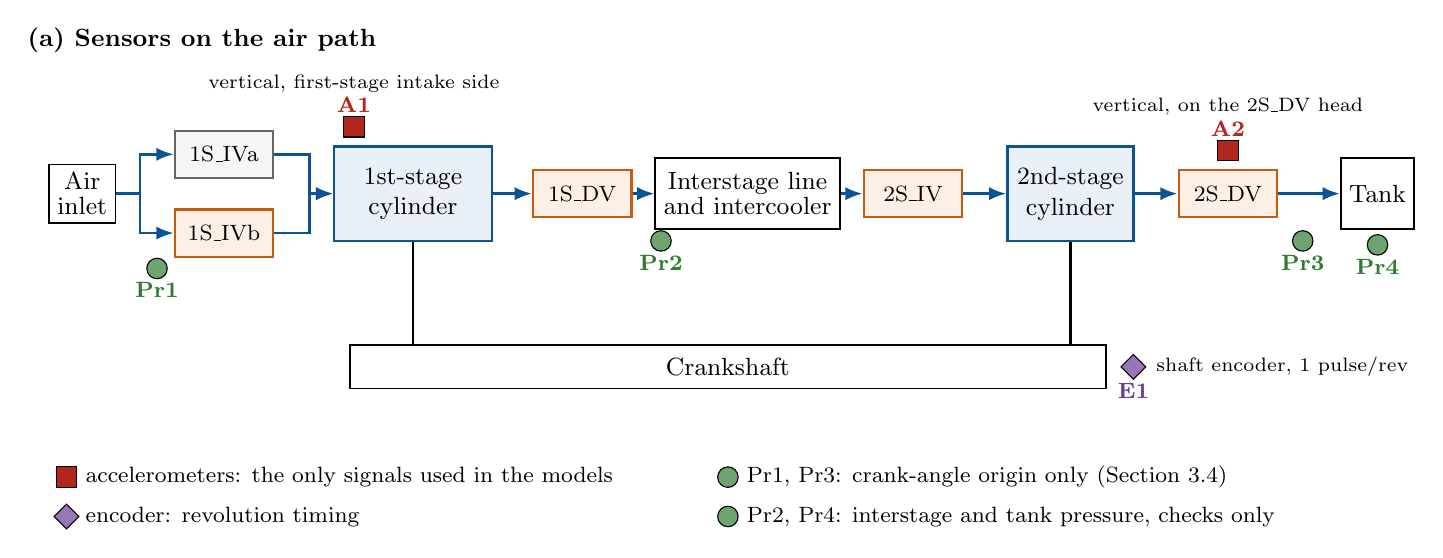
\begin{tikzpicture}[x=1cm,y=1cm]
\node[ttl] at (-0.3,3.55) {(a) Sensors on the air path};
\node[dat,minimum height=0.7cm] (in) at (0.4,1.6) {Air\\[-2pt]inlet};
\node[vlh] (iva) at (2.2,2.1) {1S\_IVa};
\node[vlv] (ivb) at (2.2,1.1) {1S\_IVb};
\node[cyl] (c1) at (4.6,1.6) {1st-stage\\cylinder};
\node[vlv] (dv1) at (6.75,1.6) {1S\_DV};
\node[dat,minimum height=0.9cm] (ic) at (8.85,1.6) {Interstage line\\[-2pt]and intercooler};
\node[vlv] (iv2) at (10.95,1.6) {2S\_IV};
\node[cyl,minimum width=1.6cm] (c2) at (12.95,1.6) {2nd-stage\\cylinder};
\node[vlv] (dv2) at (14.95,1.6) {2S\_DV};
\node[dat,minimum height=0.9cm] (tk) at (16.85,1.6) {Tank};
\draw[flow] (in.east)--++(0.3,0)|-(iva.west); \draw[flow] (in.east)--++(0.3,0)|-(ivb.west);
\draw[flow] (iva.east)-|([xshift=-3mm]c1.west)--(c1.west); \draw[flow] (ivb.east)-|([xshift=-3mm]c1.west)--(c1.west);
\draw[flow] (c1)--(dv1); \draw[flow] (dv1)--(ic); \draw[flow] (ic)--(iv2); \draw[flow] (iv2)--(c2); \draw[flow] (c2)--(dv2); \draw[flow] (dv2)--(tk);
\node[dat,minimum width=9.6cm,minimum height=0.55cm] (cs) at (8.6,-0.6) {Crankshaft};
\draw[line width=0.8pt] (c1.south)--(c1.south|-cs.north); \draw[line width=0.8pt] (c2.south)--(c2.south|-cs.north);
% accelerometers
\node[acc] (a1) at (3.85,2.45) {}; \node[sl,text=red,anchor=south] at (a1.north) {A1};
\node[lab,anchor=south,align=center] at (3.85,2.85) {\scriptsize vertical, first-stage intake side};
\node[acc] (a2) at (14.95,2.15) {}; \node[sl,text=red,anchor=south] at (a2.north) {A2};
\node[lab,anchor=south,align=center] at (14.95,2.55) {\scriptsize vertical, on the 2S\_DV head};
% encoder
\node[enc] (e1) at (13.75,-0.6) {}; \node[sl,text=pur,anchor=north] at (e1.south) {E1};
\node[lab,anchor=west] at (14.0,-0.6) {\scriptsize shaft encoder, 1 pulse/rev};
% pressures
\node[prs] (p1) at (1.35,0.65) {}; \node[sl,text=grn,anchor=north] at (p1.south) {Pr1};
\node[prs] (p2) at (7.75,1.0) {}; \node[sl,text=grn,anchor=north] at (p2.south) {Pr2};
\node[prs] (p3) at (15.9,1.0) {}; \node[sl,text=grn,anchor=north] at (p3.south) {Pr3};
\node[prs] (p4) at (16.85,0.95) {}; \node[sl,text=grn,anchor=north] at (p4.south) {Pr4};
% legend
\begin{scope}[shift={(0,-2.0)}]
\node[acc] at (0.2,0) {}; \node[lab,anchor=west] at (0.4,0) {accelerometers: the only signals used in the models};
\node[enc] at (0.2,-0.5) {}; \node[lab,anchor=west] at (0.4,-0.5) {encoder: revolution timing};
\node[prs] at (8.6,0) {}; \node[lab,anchor=west] at (8.8,0) {Pr1, Pr3: crank-angle origin only (Section 3.4)};
\node[prs] at (8.6,-0.5) {}; \node[lab,anchor=west] at (8.8,-0.5) {Pr2, Pr4: interstage and tank pressure, checks only};
\end{scope}
\end{tikzpicture}\end{document}
